\section{Introdução}

\begin{frame}
  \frametitle{Projeto Internacional}
   \begin{tcolorbox}[colback=blue!5,colframe=blue!40!black,title=Projeto Internacional]
    \textit{``Energy, air pollution, and health in developing countries``}
             coordenado pelo Dr. Majid Ezzati na \textit{Harvard School of Public Health}.
   \end{tcolorbox}
   
   \begin{tcolorbox}[colback=blue!5,colframe=blue!40!black,title=Mestrado em Nima]
      Analisar por XRF e BC rapidamente e com qualidade 3000 amostras coletadas (2006-2008) em Gana. 
      Sendo que, as referentes ao bairro de Nima, em Acra, aproximadamente 800, foram objeto de pesquisa desse Mestrado.
   \end{tcolorbox}
  
\end{frame}

\begin{frame}
  \frametitle{África}
  \begin{figure}[H]
  \centering
  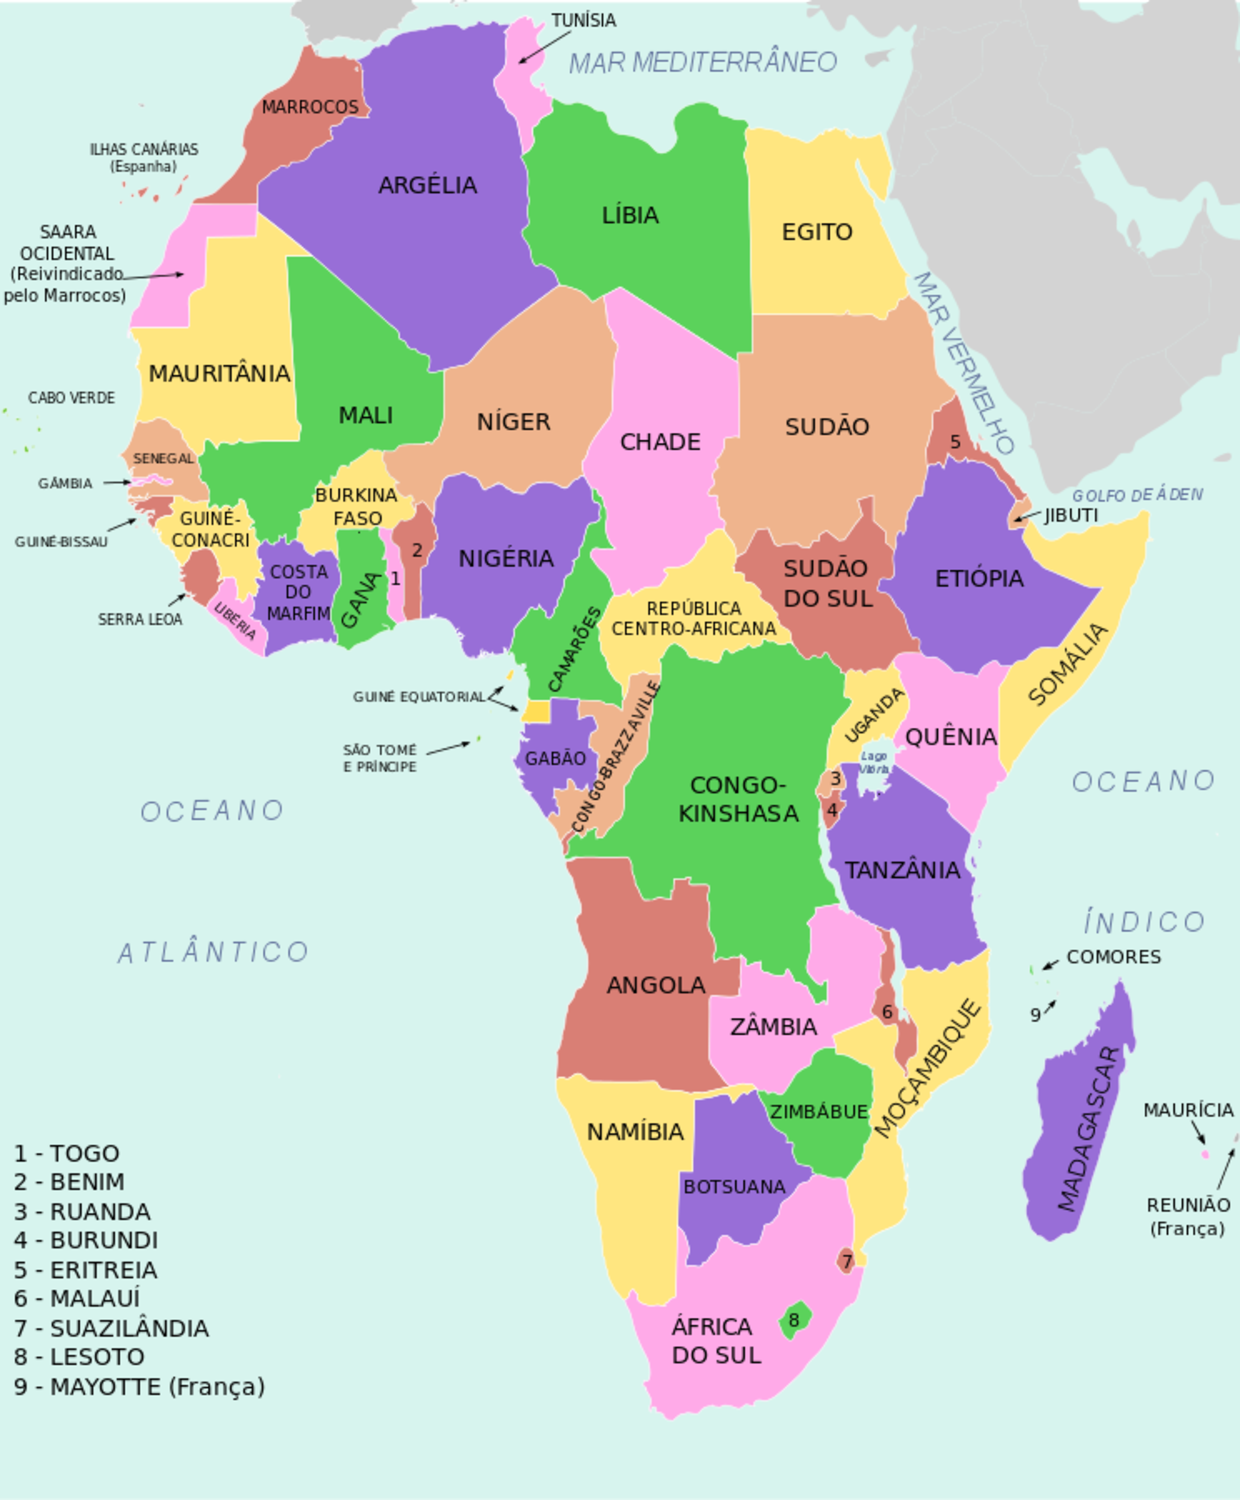
\includegraphics[width=0.55\linewidth]{../../inputs/images/africa_wikipedia.pdf}
  \end{figure}
\end{frame}

\begin{frame}
  \frametitle{África}
   \begin{itemize}
     \item Terceiro maior continente (extensão);
     \item Segundo maior em população, com 1,2 bilhões de habitantes (2015);
     \item 54 países (os mais pobres do mundo);
     \item Norte e Sul (África Subsariana - SSA) separados pelo deserto o Saara;
     \item Recente urbanização;
   \end{itemize}
\end{frame}

\begin{frame}
  \frametitle{Impactos na poluição do ar em cidades da SSA}
  \begin{itemize}
    \item População predominantemente rural, mas em transição;
    \item Excesso de vias não pavimentadas, mesmo nos centros das cidades;
    \item Alta taxa de crescimento populacional, sem a correspondente melhoria 
        na infraestrutura de serviços públicos;
    \item Emprego de queima de biomassa ou de lixo a céu aberto;
    \item Inexistência de sistemas de monitoramento de parâmetros ambientais, sistemáticos e em larga escala,
        realizados por agências de controle.
  \end{itemize}
\end{frame}

\begin{frame}
	\frametitle{Região Metropolitana de Acra (RMA)}
	  \begin{itemize}
	  	\item Acra é capital de Gana desde 1957 (independência da Inglaterra);
	  	\item Região portuária desde a colonização;
	  	\item Região litorânea com elevações que variam entre 0 e 60 metros do nível do mar;
	  	\item 4 milhões de habitantes e densidade populacional de 	  	1205 $habitantes/km^2$
	  	\item Com economia baseada majoritariamente na indústria e em serviços, 90,5\% da 
	  	população da RMA está alocada em área urbana
	  	\item (DVLA), registrou em 2009 cerca de 1,13
	  	milhões de veículos
	  	
	  \end{itemize}
\end{frame}

\begin{frame}
  \frametitle{Nima}
  \begin{center}
  Queima de lixo a céu aberto em Nima:
  \end{center}
  \begin{figure}[H]
    \centering
      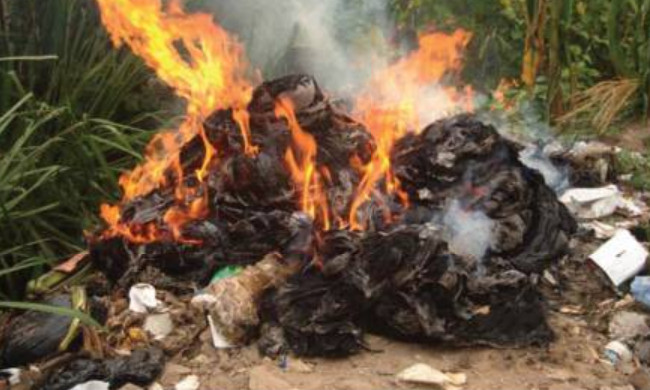
\includegraphics[width=0.5\linewidth]{../../inputs/images/zheng/arku3.jpeg}
  \end{figure} 
\end{frame}

\begin{frame}
  \frametitle{Acra}
  Foto do depósito de lixo eletrônico \textit{(e-waste)} situado no bairro 
  de Agbogbloshie em Acra.
  \begin{figure}[H]
    \centering
    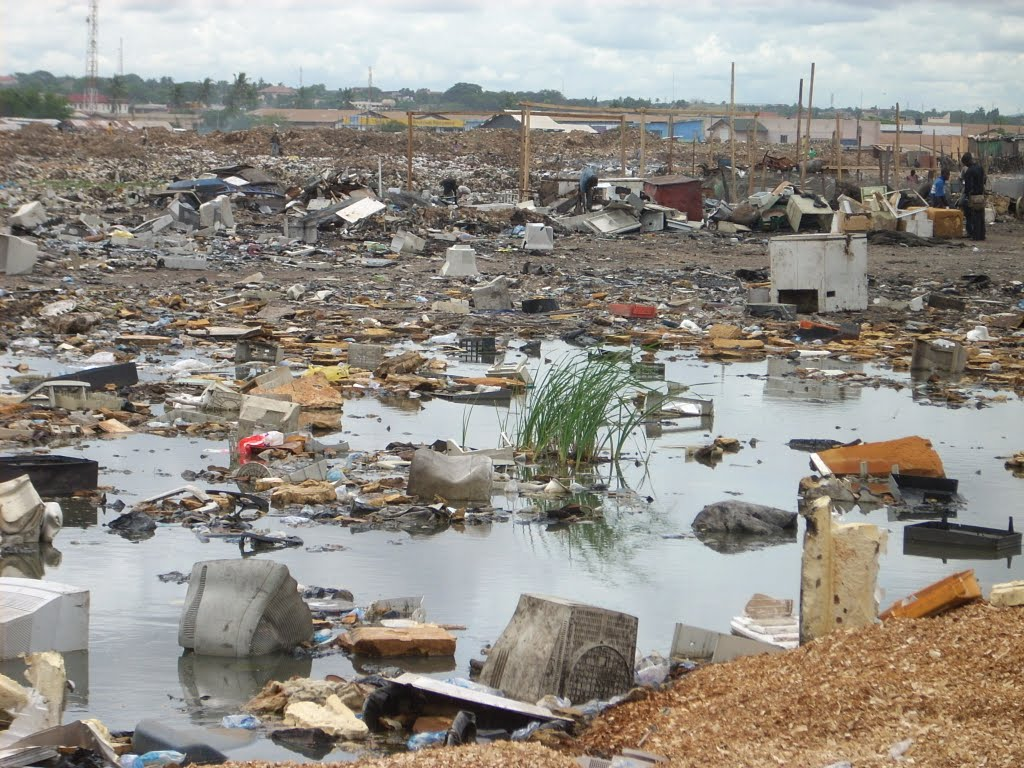
\includegraphics[width=0.5\textwidth]{../../inputs/images/ewaste_jack_caravano.jpg}
  \end{figure}
\end{frame}

\begin{frame}
  \frametitle{}
  \begin{figure}[H]
    \centering
    \begin{subfigure}[b]{0.4\linewidth}
      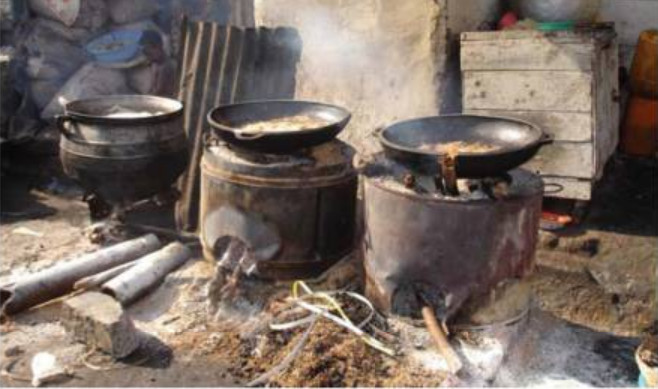
\includegraphics[width=\linewidth]{../../inputs/images/zheng/arku1.jpeg}
      \caption{Cozinha residencial em Nima adaptada para o uso de lenha.}
    \end{subfigure}%
    \hspace{0.5cm}
    \begin{subfigure}[b]{0.4\linewidth}
      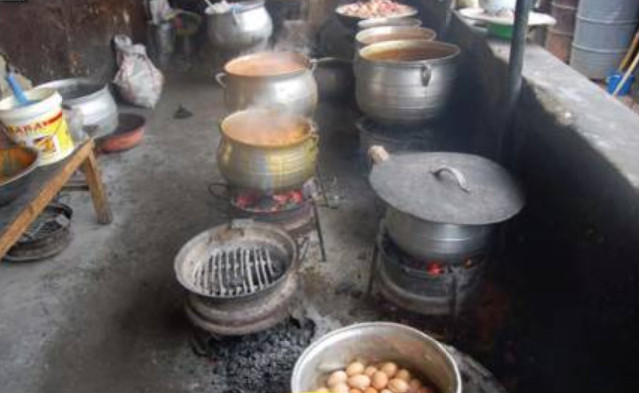
\includegraphics[width=\linewidth]{../../inputs/images/zheng/arku2.jpeg}
      \caption{Cozinha de comércio em Nima adaptada para o uso de carvão.}
    \end{subfigure}
  \end{figure}
\end{frame}